\documentclass{article}

\usepackage{polski}
\usepackage[utf8]{inputenc}
\usepackage{graphicx}

\begin{document}

\title{Steve Backley}
\author{Filip Kowalewski}
\date{}
\maketitle

Steve backley (ur. 12 lutego 1969 w Sidcup) – brytyjski lekkoatleta specjalizujący się w rzucie oszczepem.\\
Backley był jednym z najwybitniejszych oszczepników lat 90. XX wieku. Pierwszy sukces odniósł w 1987, gdy został mistrzem Europy juniorów, rok później ustanowił rekord świata juniorów (79,50)[1]. Czterokrotny mistrz Europy, trzykrotny medalista olimpijski i dwukrotny wicemistrz świata. Dwa razy bił rekord świata – 2 lipca 1990 w Sztokholmie uzyskał wynik 89,58, a dwa lata później – 25 stycznia 1992 w Auckland – uzyskał wynik 91,46 i jako pierwszy człowiek rzucił oszczepem nowego typu ponad 90 metrów. Do dziś jest to rekord Wielkiej Brytanii.\\
Odznaczony Orderem Imperium Brytyjskiego. Wystąpił w trzeciej serii brytyjskiego show Dancing on Ice, gdzie zajął 7. lokatę.\\
\\

Na zdjęciu \ref{fig:2} Steve szykuje sie to rzutu oszczepem.


\tableofcontents

\section{Osiągnięcia}

W tabeli \ref{fig:tabela} sa wypisane wszystkie osiągnięcia.




\section{Rekord świata}
In July 1990, Backley set a world record of 89.58m in Stockholm, Sweden.[3] The record was then bettered by the Czech thrower Jan Železný a few weeks later, but Backley then regained the record with a throw 90.98m at Crystal Palace, London, to end the year as the world record holder. Finland's Seppo Räty then bettered the record in 1991. The records set by Železný and Räty, as well as Backley's 90.98m throw, had all been made using new 'Nemeth' javelins, however in August 1991 the IAAF declared this type of javelin illegal and all records set using them were retrospectively deleted. As a consequence, the world record reverted to the 89.58m mark that Backley had set in 1990. Backley then set another world record of 91.46m in January 1992 in New Zealand, a record which stood until the following year when it was bettered by Zelazny.


\section{Biografia}
Backley was educated at Hurst Primary School, Bexley, and later at Bexley and Erith Technical High School for Boys (now Beths Grammar School) in his teens. He competed for Bexley in the London Youth Games.[2] He enrolled at Loughborough University in October 1988 to study for a BSc Honours degree in Physical Education, Sports Science and Recreation Management. Although he completed his first year there and remained a student until 2002, the time he dedicated to the javelin prevented him from completing his studies. However, on 16 December 2002 Loughborough University honoured him with the degree of Doctor of Technology honoris causa.\\

Backley's first significant title, was won in 1987 when he threw 75.14 metres to pick up the European junior title, ahead of Vladimir Sasimovich (73.24) of Russia and East German Raymond Hecht (72.78). In 1988, Backley won the silver medal at the 1988 World Junior Championships. He also broke the world junior record that year.

\section{Zdjęcia}


\begin{figure}
\centering
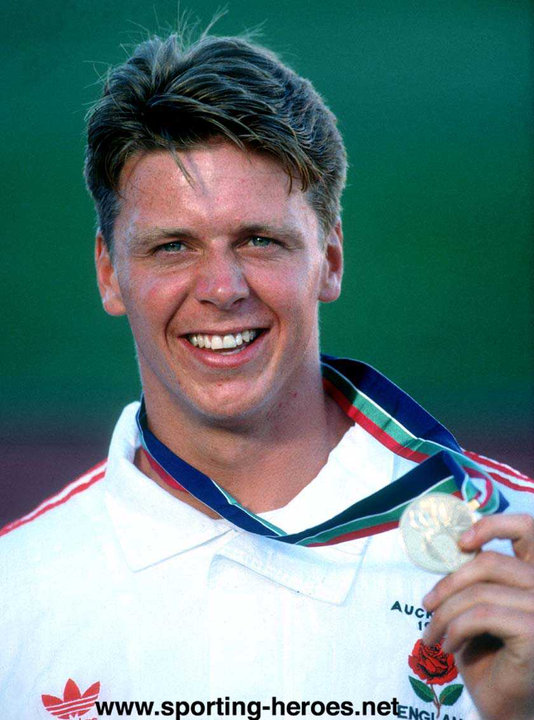
\includegraphics[width=0.5\hsize]{1.jpg}
\caption{uśmiech}\label{fig:1}
\end{figure}

\begin{figure}
\centering
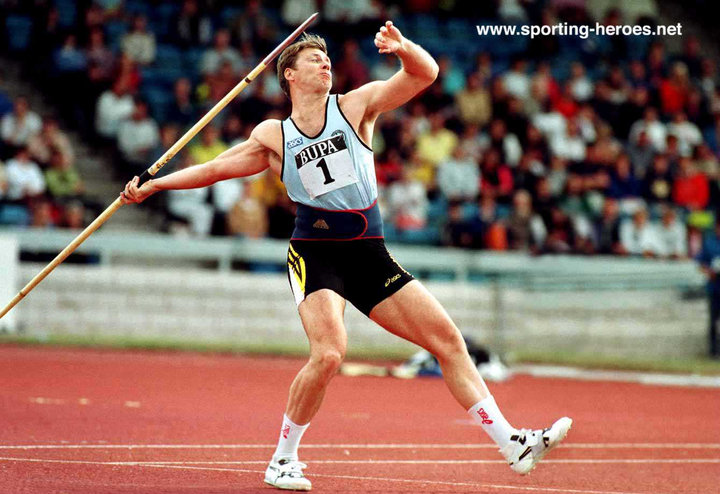
\includegraphics[width=0.5\hsize]{2.jpg}
\caption{Rzut}\label{fig:2}
\end{figure}

\begin{figure}
\centering
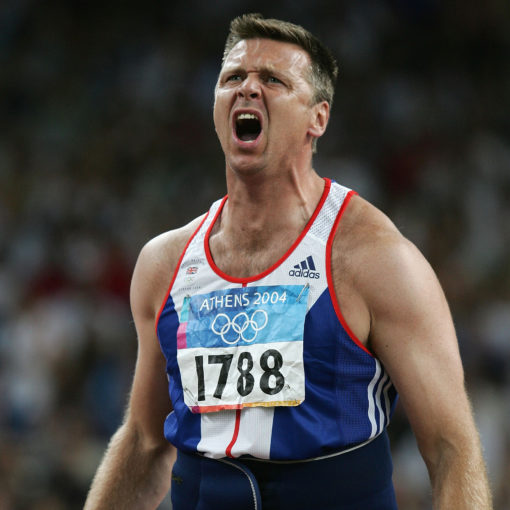
\includegraphics[width=0.1\hsize]{3.jpg}
\caption{okrzyk}\label{fig:3}
\end{figure}

\begin{table}



\begin{tabular}{lcccc}
\textbf{Rok}&\textbf{Impreza}&\textbf{Miesjce}&\textbf{Lokata}&\textbf{Wynik}\\
\hline
1987&Mistrzostwa Europy juniorów&Birmingham&1. miejsce&75{,}14\\
1988&Mistrzostwa Świata juniorów&Greater Sudbury&2. miejsce&75{,}40\\
1989&Finał A pucharu Europy&Gateshead&1. miejsce&82{,}92\\
1989&Puchar świata&Barcelona&1. miejsce&85{,}90\\
1989&Uniwersjada&Duisburg&1. miejsce&85{,}60\\
1990&Mistrzostwa Europy&Split&1. miejsce&87{,}30\\
1990&Igrzyska Wspólnoty Narodów&Auckland&1. miejsce&86{,}02\\
1991&Uniwersjada&Sheffield&1. miejsce&87{,}42\\
1991&Mistrzostwa świata&Tokio&15. miejsce&78{,}24\\
\hline


\end{tabular}
\caption{tabela medali}
\label{fig:tabela}
\end{table}


\end{document}